\documentclass{article}
\usepackage[colorlinks = true,
            linkcolor = blue,
            urlcolor  = blue,
            citecolor = blue,
            anchorcolor = blue]{hyperref}
\usepackage{graphicx}
\usepackage[parfill]{parskip}
\usepackage[margin=1in]{geometry}
\usepackage{titling}

\graphicspath{{images/}}
\pagenumbering{gobble}
\title{Raytracing Project}
\author{Jared Givens, Ahbi Sohal, Noah Krim}
\date{28 May, 2023}

\pretitle{% add some rules
  \begin{flushleft}
    \Large
    \bfseries
    % \Huge\bfseries
}%, make the fonts bigger, make the title (only) bold
\posttitle{%
  \end{flushleft}%
}
\preauthor{%
  \begin{flushleft}
    \begin{tabular}[t]{@{}l@{}}%
}
\postauthor{%
    \end{tabular}
  \end{flushleft}%
}
\predate{%
  \begin{flushleft}
}
\postdate{%
  \end{flushleft}%
}


\begin{document}
\maketitle

\large
Description

\normalsize
The program outputs color values of pixels with raytracing techniques. 
It begins by initializing virtual geometry and a camera. Then it sends rays from the camera 
into the virtual space. 

For each pixel, a series of uniformly random rays are 
cast to gather a color value. The color values are then averaged to achieve anti-aliasing. 

Each ray iterates over the scene's geometry to determine the nearest 
intersection. The nearest intersection's color is multiplied against the 
rays running total color value. The ray then reflects and scatters or refracts 
based on the properties of the intersected material. The process of 
accumulating color and bouncing continues until the ray fails to collide with 
an object or reaches the maximum ray depth. If the ray fails to collide, the 
program adds the contribution of the skybox to complete the color.  
If the ray reaches the 
maximum bounce depth, the color is set to black.  

\large
Qualification

\normalsize
Our team will be able to complete this project because we have significant experience working with linear
algebra and systems programming languages. Our team was able to complete the 
\href{https://github.com/abhiss/lstore}
{ECS165 L-Store Database Project} 
Project in Rust. Furthermore, we have already made significant progress on our 
\href{https://github.com/JaredGivens/ECS158-Raytracing}{Serial Prototype}
. There are also
significant online resources on raytracing, including the guide we referenced to build our prototype:
\href{https://raytracing.github.io/books/RayTracingInOneWeekend.html}{Ray Tracing in One Weekend}.

\large
Justification

\normalsize
Our serial prototype output a single frame in 5.971 seconds
(wall-clock time 2020 Macboock 2 GHz). This program is an excellent 
candidate for CUDA because the code for each ray can run in parallel. 
Currently, most of the time is spent computing the ray intersections and bounces, which 
have no data dependencies. Additionally, the majority of code is linear algebra 
with few branches. Some of the branches could be removed with different equations. 
One of the largest issues with ray tracing is determining which geometry can be 
intersected by a given ray, and we may need to implement a tree structure to 
determine hit candidates efficiently. If time permits, we have plans to add 
support for triangles, lights, and textures.

Here is a frame from the serial prototype:

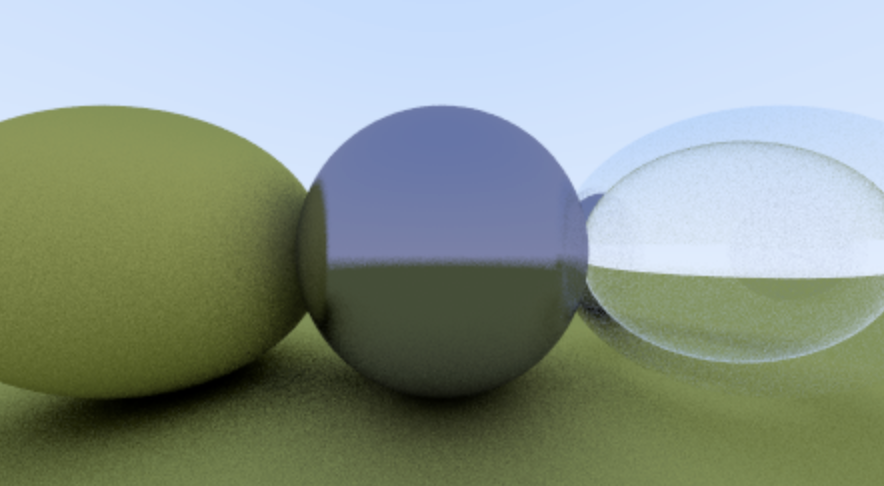
\includegraphics[scale=0.6]{rtsc}

\end{document}.